\documentclass[journal]{journal}
\usepackage[margin=1in]{geometry}
\usepackage{verbatim}
\usepackage[justification=centering]{subfig}
\usepackage{graphicx}
\usepackage{url} % typeset URL's reasonably
\usepackage{listings}
\usepackage[colorlinks]{hyperref}
\usepackage{pslatex} % Use Postscript fonts
\usepackage{algorithm}
\usepackage{algpseudocode}
%\usepackage[]{algorithm2e}
%\usepackage{subcaption}
\usepackage{color}
\usepackage{multirow}
\usepackage{makecell}

\usepackage{mathptmx}
\usepackage{amsmath}

%\usepackage{appendix}
%define some own functions

\newenvironment{mycell}[1]
{
	\begin{minipage}{#1}
		\begin{center}
			\vspace*{0.15cm}
		}
		{
			\vspace*{0.1cm}
		\end{center}
	\end{minipage}
}

\newcommand{\tabincell}[2]{\begin{tabular}{@{}#1@{}}#2\end{tabular}} 
\def\D{\mathrm{d}}

\begin{document}

	\title{Towards the Robust Image Recognition Using Spiking Neurons}
	\author{
	Qian~Liu
	\thanks{
	The author is with the School of Computer Science, University of Manchester, Manchester M13 9PL, U.K. 
	(e-mail:qian.liu-3@manchester.ac.uk}
	}
	\maketitle
	\thispagestyle{empty}

\begin{abstract}

\end{abstract}

\section{Introduction}
	To gain a better understanding of the brain and build biologically-inspired computers, increasing attention is being paid to research into spike-based neural computation.
	Within the field, the visual pathway and its hierarchical organisation have been extensively studied within the primate brain.
	Spiking Neural Networks (SNNs) inspired by the understanding of observed biological structure and function have been successfully applied to visual recognition/classification tasks.
	In addition, implementations on neuromorhpic hardware have made large-scale networks run in (or even faster than) real time, and accessible on mobile robots.
	Neuromorphic sensors, e.g. silicon retinas, are able to feed such a mobile system with real-time visual stimuli.
	A new series of vision benchmarks for spike-based neural processing are now needed to quantitatively measure progress within this rapidly advancing field.
	We propose that a large dataset of spike-based visual stimuli is needed to provide a baseline for comparisons on SNN models and algorithms, and some benchmarking network models are also required to validate the accuracy and cost of these neuromorphic hardware platforms.
	
	First of all, an initial NE (Neuromorphic Engineering) dataset of input stimuli based on standard computer vision benchmarks consisting of %facial images (FERET database) and 
	digits (from the MNIST database) is presented according to the current research on spike-based image recognition.
	Within this dataset, all images are centre aligned and having similar scale.
	We describe how we intend to expand this dataset to fulfil the needs of upcoming research problems.
	For instance, the data should provide cases to measure position-, scale-, and viewing-angle invariance.
	The data are in Address-Event Representation (AER) format which is widely used in the neuromorphic engineering field unlike conventional images.
	These spike trains are produced by various techniques: rate-based Poisson spike generation, rank order encoding and recorded output from a silicon retina with both flashing and oscillating input stimuli.
	Furthermore a complementary evaluation methodology is also presented to assess both model-level and hardware-level performance.
	% and to benchmark hardware systems with two example models.
	%An evaluation methodology is also presented which describes how to consistently assess the performance of a SNN model and its cost implemented on neuromorphic hardware.
	Finally, we provide two SNN models to validate their classification capabilities and to assess the performances of their hardware implementations as tentative benchmarks.
	%The network is trained on-line using the Spike Timing Dependent Plasticity (STDP) learning rule on a massive-parallel neuromorphic simulator, e.g. SpiNNaker.
	
	With this dataset we hope to (1) promote meaningful comparison between algorithms in the field of neural computation, (2) allow comparison with conventional image recognition methods, (3) provide an assessment of the state of the art in spike-based visual recognition, and (4) help researchers identify future directions and advance the field.
	
	SDBN
%	\subsection{Motivation}
%	\subsection{State-of-the-art}
%	\subsection{Problems}
\section{Related Works}
	\cite{riesenhuber1999hierarchical} proposed a quantitative modelling framework of object recognition with position-, scale- and view-invariance based on the units of MAX-like operations.
	The cortical-like model has been analysed on several datasets~\cite{serre2007robust}.
	And recently~\cite{fu2012spiking} reported that their SNN implementation of the framework was capable of facial expression recognition with a classification accuracy (CA) of 97.35\% on the JAFFE dataset~\cite{lyons1998coding} which contains 213 images of 7 facial expressions posed by 10 individuals.
	% 97.35\% on JAFFE dataset.
	They employed simple integrate-and-fire neurons with rank order coding (ROC) where  the earliest pre-synaptic spikes have the strongest impact on the post synaptic potentials.
	According to~\cite{vanrullen2002surfing}, the first wave of spikes  carry explicit information through the ventral stream and in each stage meaningful information is extracted and spikes are regenerated. 
	Using one spike per neuron,~\cite{delorme2001face} reported 100\% and 97.5\% accuracies on the face identification task over changing  contrast and luminance training (40 individuals $\times$ 8 images) and testing data (40 individuals $\times$ 2 images) respectively.
	%These developments yielded a large number of papers on SNNs based recognition, with a majority reporting outstanding recognition resulton limited-size databases.
	
	The Convolutional Neural Network (CNN), also known as the \textit{ConvNet} developed by~\cite{lecun1998gradient}, is a well applied model of such a cortex-like framework.
	%Reported results:
	%Hand Gestures, Qian Liu
	An early Convolutional Spiking Neural Network (CSNN) model identified faces of 35 persons with a CA of 98.3\% exploiting simple integrate and fire neurons~\cite{matsugu2002convolutional}.
	Another CSNN model~\cite{zhao2014feedforward} was trained and tested both with DVS raw data and Leaky Integrate-and-Fire (LIF) neurons.
	%The MAX operation, training and the switch are not only neuron involved.
	It was capable of recognising three moving postures with a CA of about 99.48\% and 88.14\% on the MNIST-DVS dataset (see Chapter~\ref{sec:data}).
	As one step forward,~\cite{camunas2012event} implemented a convolution processor module in hardware which could be combined with a DVS for high-speed recognition tasks.
	The inputs of the ConvNet were continuous spike events instead of static images or frame-based videos. 
	The chip detected four suits of a 52 card deck while the cards were fast browsed in only 410 ms.
	Similarly, a real-time gesture recognition model~\cite{liu2014real} was implemented on a neuromorphic system with a DVS as a front-end and a SpiNNaker~\cite{furber2014spinnaker} machine as the back-end where LIF neurons built up the ConvNet configured with biological parameters.
	In this study's largest configuration, a network of 74,210 neurons and 15,216,512 synapses used 290 SpiNNaker cores in parallel and reached 93.0\% accuracy. 
	
	Deep Neural Networks (DNNs) together with deep learning are the most exciting research fields in vision recognition.
	The spiking deep network has great potential to combine remarkable performance with the energy efficient training and running.
	In the initial stage of the research, the study was focused on converting off-line trained deep network to SNNs~\cite{o2013real}.
	The same network initially implemented on a FPGA achieved a CA of 92.0\%~\cite{neil2014minitaur}, while a later implementation on SpiNNaker scored 95.0\%~\cite{Stromatias2015scalable}.
	%The performance was increased from 92.0\% to 95.0\%~\cite{Stromatias2015scalable} by implementing the model on SpiNNaker instead of the earlier FPGA version.
	Recent attempts have contributed to better translation by utilising modified units in a ConvNet~\cite{cao2015spiking} and tuning the weights and thresholds~\cite{Diehl2015fast}).
	The later paper claims a state-of-the-art performance (99.1\% on the MNIST dataset) comparing to original ConvNet.
	The current trend of training Spiking DNNs on-line using biologically-plausible learning methods is also promising.
	An event driven Contrastive Divergence (CD) training algorithm for RBMs (Restricted Boltzmann Machines) was proposed for Deep Belief Networks (DBN) using LIF neurons with STDP (Spike-Timing-Dependent Plasticity) synapses and verified on MNIST (91.9\%)~\cite{neftci2013event}.
	
	STDP as a biological learning process is applied to vision tasks.
	\cite{bichler2012extraction} demonstrated an unsupervised STDP learning model to classify car trajectories captured with a DVS retina. 
	A similar model was tested on a Poissonian spike presentation of the MNIST dataset achieving a performance of 95.0\%~\cite{diehl2015unsupervised}.
	Theoretical analysis~\cite{nessler2013bayesian} showed that unsupervised STDP was able to approximate a stochastic version of Expectation Maximization, a powerful learning algorithm in machine learning.
	The computer simulation achieved~93.3\% CA on MNIST and could be implemented in a memrisitve device~\cite{bill2014compound}. 
	
\section{Benchmarking spike-based visual recognition}
	%Experiment setup/ collection method/ properties of each class/ etc.
	The name of the first proposed dataset in the benchmarking system is NE15-MNIST which stands for Neuromorphic Engineering 2015 on MNIST.
	The original MNIST dataset is downloaded from the website\footnote{http://yann.lecun.com/exdb/mnist/} of THE MNIST DATABASE of handwritten digits~\cite{lecun1998gradient}.
	The NE15-MNIST is converted into a spiking version of the original dataset consisting of four subsets which were generated for different purposes:
	\begin{itemize}
		\item \textit{Poissonian}
		to benchmarking existing methods of rate-based spiking models.
		\item \textit{FoCal}
		to promote the study of spatio-temporal algorithms applied to recognition tasks using few input spikes.
		\item \textit{DVS recorded flashing input}
		to encourage research on fast recognition methods which are found in the primate visual pathway.
		\item \textit{DVS recorded moving input}
		to trigger the study of algorithms targeting on continuous input from real-world sensors and to implement them on mobile neuromorphic robots.
	\end{itemize}
	The dataset can be found in the GitHub repository at: https://github.com/qian-liu/benchmarking.
	\subsection{The Dataset: NE15-MNIST}
	\subsubsection{File~Formats}
	
	Two file formats are supported in the dataset: jAER format~\cite{delbruck2008frame} (.dat or .aedat), and binary file in NumPy .npy format.
	The  address event representation (AER) interface has been widely used in neuromorphic systems, especially for vision sensors.
	The spikes are encoded as time events with corresponding addresses to convey information.
	The spikes in jAER format, both recorded from a DVS retina and artificially generated, can be displayed in jAER software.
	Figure~\ref{Fig:jaer} is a snapshot of the software displaying an .aedat file which is recorded by a DVS retina~\cite{serrano2013128}.
	The resolution of the DVS recorded data is 128$\times$128.
	%, while the original MNIST data is 28$\times$28.
	The other format of spikes used is a list of spike source arrays in PyNN~\cite{davison2008pynn}, a description language for building spiking neuronal network models.
	Python code for converting one file format to and from the other is also provided.
	
	\begin{figure}[hbt]
		\centering
		\subfloat[A snapshot of jAER playing the DVS recorded spikes.]{
			\label{Fig:jaer}
			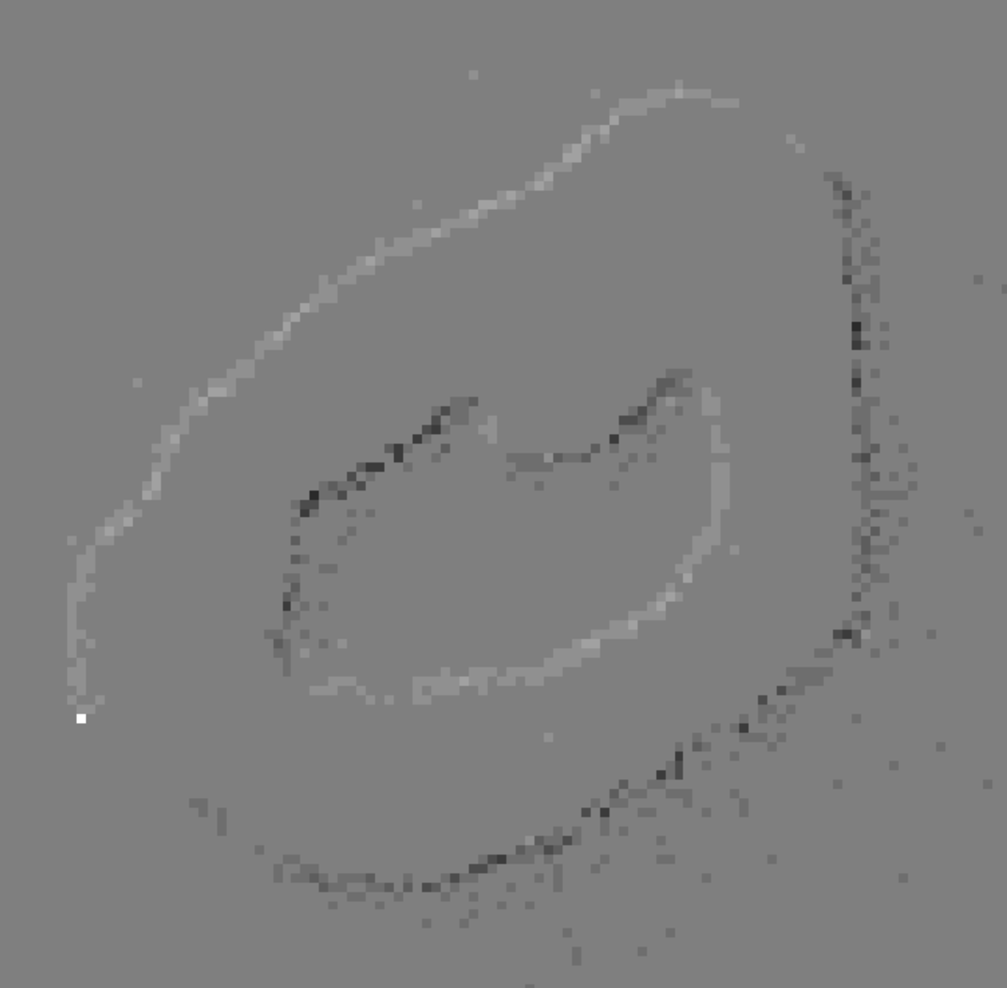
\includegraphics[width=0.22\textwidth]{images/dvs-128.pdf}
		}
		\subfloat[A snapshot of jAER playing Poissonian spike trains.]{
			\label{Fig:poisson}
			
\includegraphics[width=0.22\textwidth]{images/zero-28-2.pdf}
		}\\
		\subfloat[The raster plot of the Poissonian spike trains.]{
			\label{Fig:raster}
			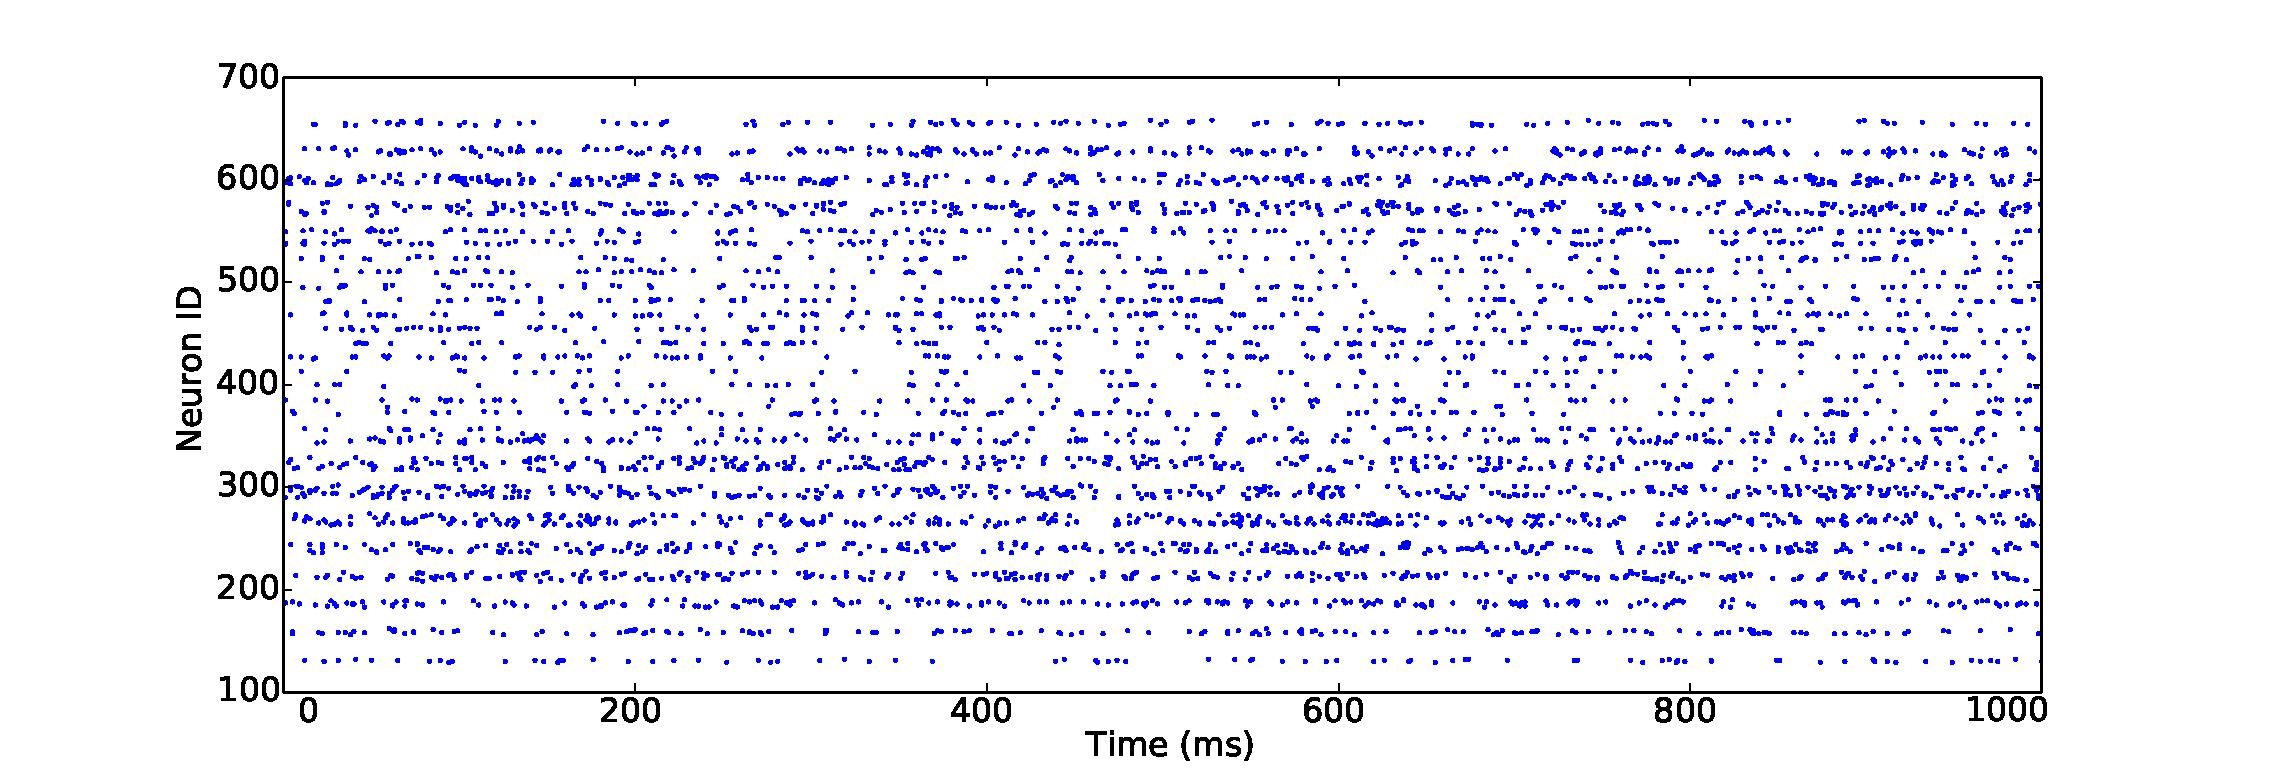
\includegraphics[width=0.48\textwidth]{images/zero.pdf}
		}
		
		\caption{
			Snapshots of jAER software playing spike presented videos.
			The same image of digit ``0'' is transformed to spikes by DVS recording and the Poissonian generation respectively.
			A raster plot of the Poissonian spike trains is also provided.}
		\label{fig:zero}
	\end{figure}
	
%	\subsection{Data Description}	
	\subsubsection{Poissonian}
	
	In the cortex, the timing of spikes is highly irregular~\cite{squire1998findings}.
	It can be interpreted that the inter-spike interval reflects a random process driven by the instantaneous firing rate.
	If the generation of each spike is assumed to be independent of all the other spikes, the spike train is seen as a Poisson process.
	The spiking rate can be estimated by averaging the pooled responses of the neurons.
	
	As stated above, rate coding is exclusively used in presenting images with spikes.
	The spiking rate of each neuron is in accordance with its corresponding pixel intensity.
	Instead of providing exact spike arrays, we share the Python code for generating the spikes.
	Every recognition system may require different spiking rates and various lengths of their durations.
	The generated Poissonian spikes can be in the formats of both jAER and PyNN spike source array.
	Thus, it is easy to visualise the digits and also to build spiking neural networks.
	Because different simulators generate random Poissonian spike trains with various mechanisms, languages and codes, using the same dataset enables performance evaluation on different simulators without the interference created by non-unified input.
	The same digit displayed in Fig.~\ref{Fig:jaer} is converted to Poissonian spike trains, see Fig.~\ref{Fig:poisson}.
	The raster plot can be found in Fig.~\ref{Fig:raster}, indicating the intensities of the pixels.
	
	
	
	\subsubsection{Rank-Order-Encoding}
	A different way of encoding spikes is using a rank-order code; this means
	keeping just the order in which those spikes were fired and disregarding the exact timing. Rank-ordered spike trains have been used in vision tasks under a biological plausibility constraint, making them a viable way of image encoding for neural applications~\cite{van2001rate,sen2009evaluating,masmoudi2010novel}.
	
	\subsubsection{DVS Sensor Output with Flashing Input}
	\label{subsec_flash}
	The purpose of including the subset of DVS recorded flashing digits is to promote the application of Rank-Order-Coding to DVS output, and accelerate the fast on-set recognition by using just the beginning part of spike trains within less than 30~ms.
	
	Each digit and a blank image was shown alternately and each display lasted one second.
	The digits were displayed on an LCD monitor in front of the DVS retina~\cite{serrano2013128} and were placed in the centre of the visual field of the camera.
	%	Each recording was cut into 10 sub sections.
	Since there are two polarities of the spikes: 'ON' indicates the increase of the intensity while 'OFF' reflects the opposite, there are 'ON' and 'OFF' flashing recordings respectively per digit.
	In Fig.~\ref{fig:flash}, the burstiness of the spikes is illustrated where most of the spikes occur in a 30~ms slot. 
	In total, the subset of the database contains 2$\times$$60,000$ recordings for training and 2$\times$$10,000$ for testing.
	%	Due to the size limit of online repositories, only the third of every sequence of flashes is published.
	
	\begin{figure}[b!]
		\centering
		\subfloat[Spikes recorded in the order of neuron ID during 1s of time.]{
			\label{fig:flash_all}
			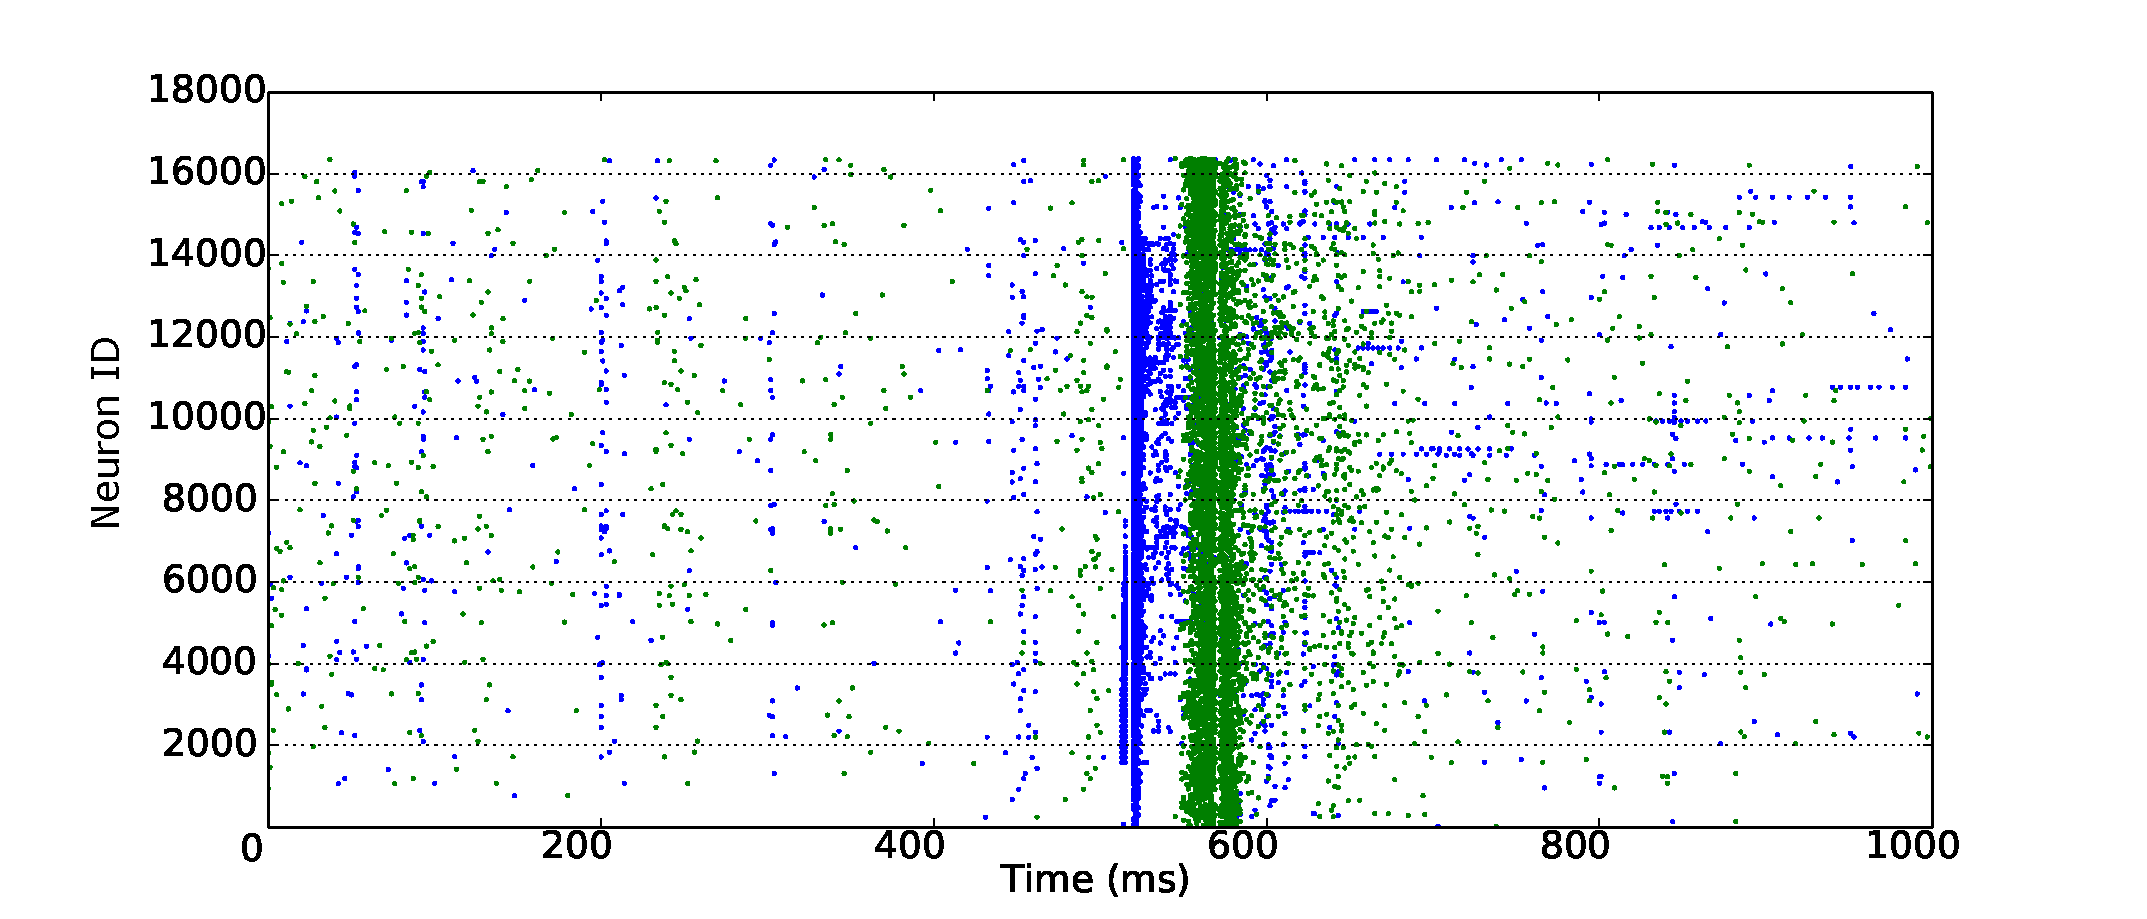
\includegraphics[width=0.48\textwidth]{images/flash_full.pdf}
		}
		\\
		\subfloat[Spikes plotted in the sequence of appearing time during 1s of time. Bursty spikes apeer in slots less than 30~ms. ]{
			\label{fig:flash_a}
			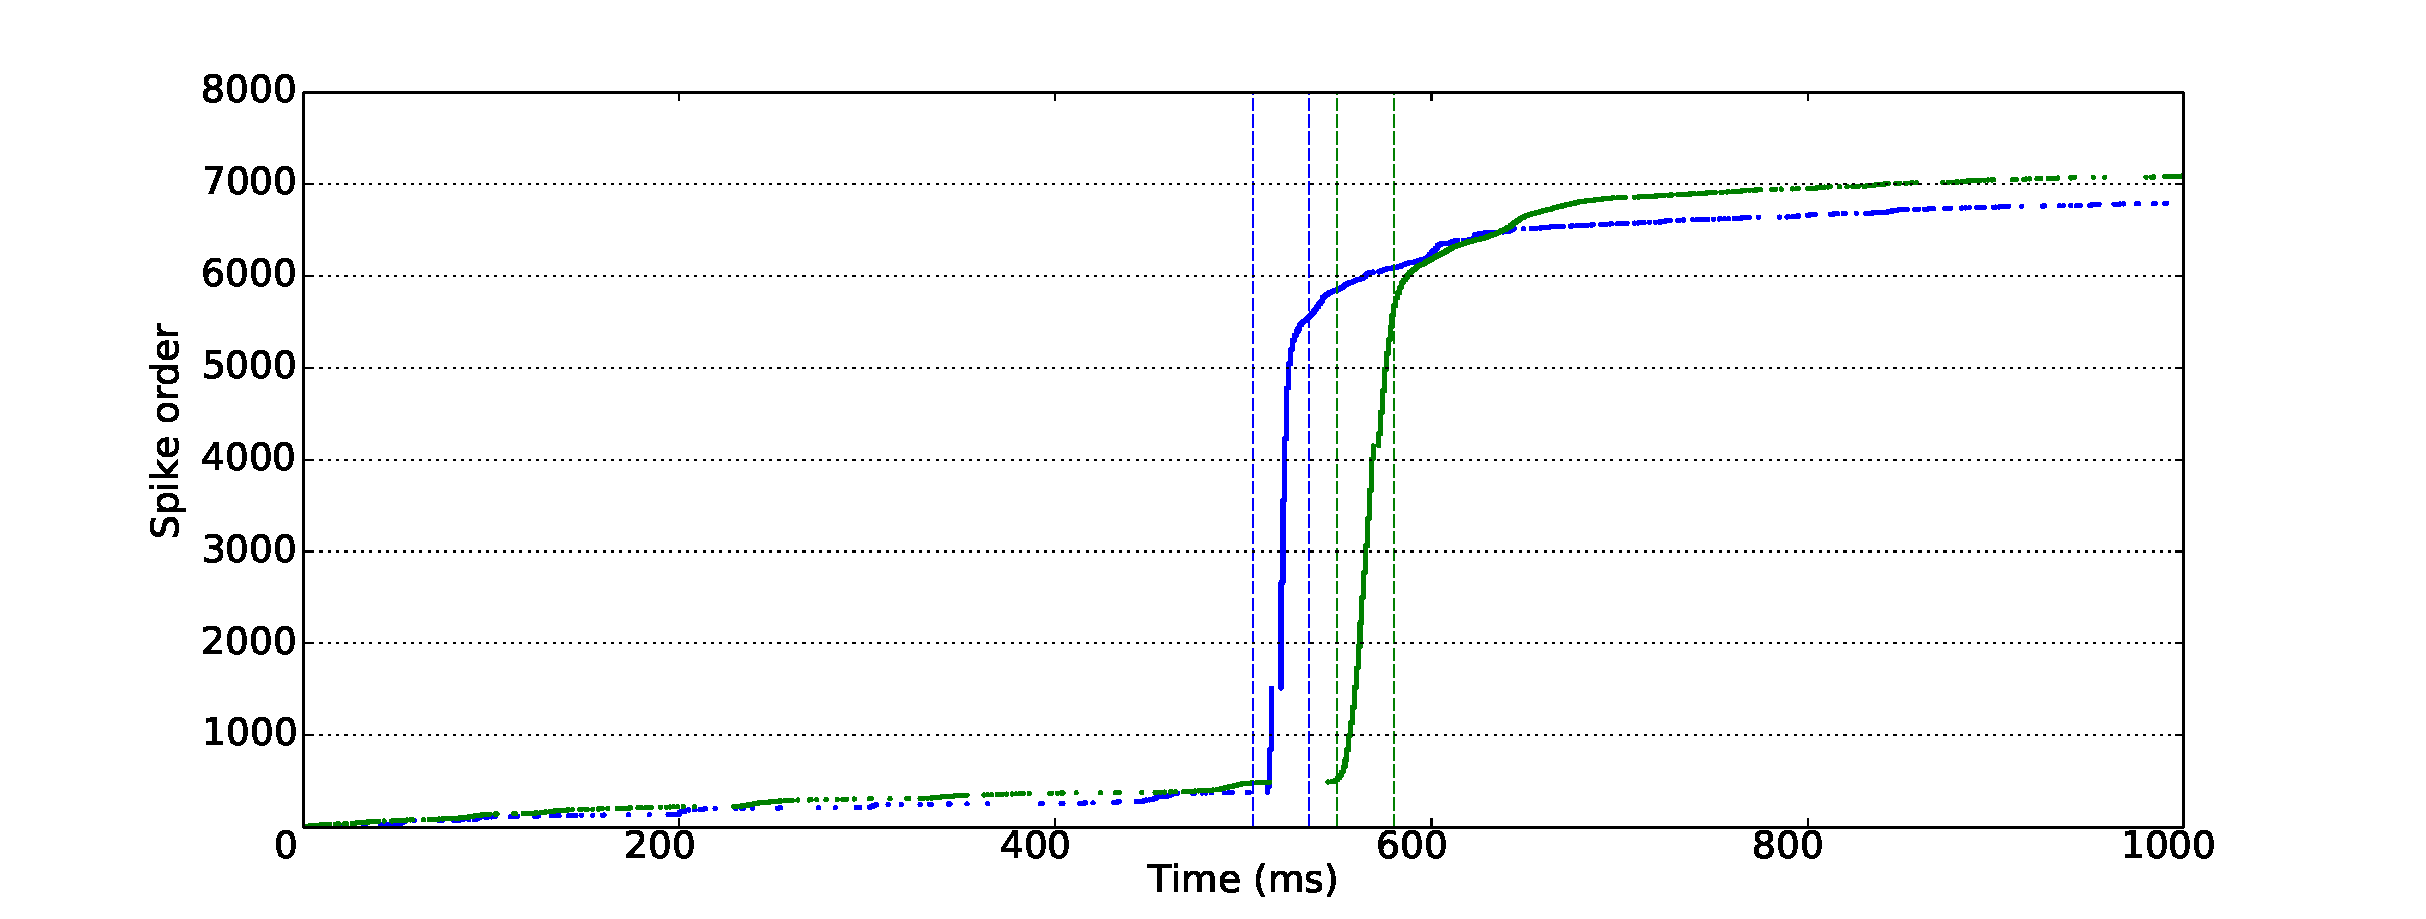
\includegraphics[width=0.48\textwidth]{images/flash_full_order.pdf}
		}
		%	  \\
		%	  \subfloat[Bursty spikes appearing in a 30~ms slot.]{
		%	  	\label{fig:flash_b}
		%	  	\includegraphics[width=0.48\textwidth]{flash_100.png}
		%	  }
		
		\caption{The bursty of spikes is illustrated where most of the spikes occur in a 30~ms slot. Blue for 'ON' events and green for 'OFF'.}
		\label{fig:flash}
	\end{figure}
	%	\subsubsection{DVS Sensor Output with Oscillating Input}
	\subsubsection{DVS Sensor Output with Moving Input}
	In order to address the problems of position- and scale- invariance, a subset of DVS recorded moving digits is presented.
	
	MNIST digits were scaled to three different sizes, by using smooth interpolation algorithms to increase their size from the original 28x28 pixel size, and displayed on the monitor with slow motion. 
	The same DVS~\cite{serrano2013128} used in Section~\ref{subsec_flash} captured the movements of the digits and generated spike trains for each pixel of its 128$\times$128 resolution.
	A total of 30,000 recordings were made: 10 digits, at 3 different scales, 1000 different handwritten samples for each.
	%	The subset is available at the website\footnote {http://imse-cnm.csic.es/caviar/MNIST\_DVS}.


	\subsection{Evaluation}
	A complementary evaluation methodology is essential to provide common metrics and assess both the model-level and hardware-level performance.

	\begin{table*}[hbt!]
		\caption{Hardware independent comparison}
		\begin{center}
			\bgroup
			\def\arraystretch{1.5}
			\begin{tabular}{ l c c c c }
				$ $ &
				\begin{mycell}{1.9cm}Preprocessing\end{mycell} & 
				\begin{mycell}{3.5cm} Network\end{mycell} & 
				\begin{mycell}{3.5cm} Training \end{mycell} & 
				\begin{mycell}{3.5cm} Recognition \end{mycell} \\
				%      \cline{3-5}
				%       & 
				%       & 
				%      \begin{mycell}{3.5cm}Topology, neuron and synapse models, \\extra classifier  \end{mycell} &
				%      \begin{mycell}{3.5cm}Methodology, simulation time, sample repetition \end{mycell} & 
				%      \begin{mycell}{3.5cm}Events/$s$, time/sample, response time, accuracy\end{mycell} \\
				\hline
				
				%
				\begin{mycell}{2.5cm}~\cite{brader2007learning} \end{mycell} & 
				\begin{mycell}{1.9cm} None \end{mycell} & % preprocessing
				\begin{mycell}{3.5cm} Two layer, LIF neurons\end{mycell}&  % network
				\begin{mycell}{3.5cm} Semi-supervised, STDP, calcium LTP/LTD\end{mycell}&  % training
				\begin{mycell}{3.5cm} 96.5\% \end{mycell} \\% recognition
				
				%
				\begin{mycell}{2.5cm}~\cite{beyeler2013categorization} \end{mycell} & 
				\begin{mycell}{1.9cm} None \end{mycell} & % preprocessing
				\begin{mycell}{3.5cm} V1 (edge), \\V4 (orientation),\\ and competitive decision, Izhikevich neurons\end{mycell}&  % network
				\begin{mycell}{3.5cm} Semi-supervised, STDP, \\ calcium LTP/LTD \end{mycell} &  % training
				\begin{mycell}{3.5cm} 91.6\% \\ 300~ms per test \end{mycell} \\% recognition
				
				%
				\begin{mycell}{2.5cm}~\cite{neftci2013event} \end{mycell} & 
				\begin{mycell}{1.9cm} Thresholding\end{mycell} & % preprocessing
				\begin{mycell}{3.5cm} Two layer RBM, \\ LIF neurons \end{mycell}&  % network
				\begin{mycell}{3.5cm} Event-driven contrastive divergence, supervised \end{mycell}&  % training
				\begin{mycell}{3.5cm} 91.9\% \\ 1~s per test\end{mycell} \\% recognition
				
				%
				\begin{mycell}{2.5cm}~\cite{diehl2015unsupervised} \end{mycell} & 
				\centering None &
				\begin{mycell}{3.5cm} Two layers, LIF neurons, inhibitory feedback  \end{mycell}& 
				\begin{mycell}{3.5cm} Unsupervised, exp. STDP, %adaptive membrane potential, 
					$3,000,000$~s of training\\ $200,000$~s per iteration\end{mycell} & 
				\begin{mycell}{3.5cm} 95\% \end{mycell}\\
				
				%
				\begin{mycell}{2.5cm}~\cite{Diehl2015fast}\end{mycell}  & 
				\begin{mycell}{1.9cm} None \end{mycell} & % preprocessing
				\begin{mycell}{3.5cm} ConvNet or \\FCnet, LIF neurons \end{mycell}& % network
				\begin{mycell}{3.5cm} Off-line trained with ReLU, weight normalization \end{mycell}&   % training
				\begin{mycell}{3.5cm} 99.1\% (ConvNet), \\ 98.6\% (FCnet);\\0.5~s per test\end{mycell}\\ % recognition    
				%
				\begin{mycell}{2.5cm}~\cite{zhao2014feedforward}\end{mycell}  & 
				\begin{mycell}{1.9cm} Thresholding\\ or DVS \end{mycell}& % preprocessing 
				\begin{mycell}{3.5cm} Simple (Gabor), \\Complex (MAX) \\and Tempotron  \end{mycell}& % network
				\begin{mycell}{3.5cm} Tempotron, supervised \end{mycell}& % training
				\begin{mycell}{3.5cm} Thresholding \\ 91.3\%, 11~s per test \\ DVS \\ 88.1\%, 2~s per test\end{mycell}\\ % recognition
				
				%
				\begin{mycell}{2.5cm} % %\cite{Stromatias2015scalable} \\ 
					This paper \end{mycell} & 
				\begin{mycell}{1.9cm} None \end{mycell} & % preprocessing
				\begin{mycell}{3.5cm} Four layer RBM, \\ LIF neurons \end{mycell}&  % network
				\begin{mycell}{3.5cm} Off-line trained, unsupervised \end{mycell}&  % training
				\begin{mycell}{3.5cm} 94.94\%\\16 ms latency \end{mycell} \\% recognition
				%
				\begin{mycell}{2.5cm} This paper \end{mycell}  & 
				\begin{mycell}{1.9cm} None \end{mycell}& % preprocessing 
				\begin{mycell}{3.5cm} FC decision layer, \\ LIF neurons \end{mycell}& % network
				\begin{mycell}{3.5cm} K-means clusters,\\Supervised STDP\\$18,000$~s of training \end{mycell}& % training
				\begin{mycell}{3.5cm} 92.98\%\\1~s per test\\10.70~ms latency\end{mycell}\\ % recognition
			\end{tabular}
			\egroup
		\end{center}
		\label{tb:software_comparison}
	\end{table*}
	
	\begin{table*}[thb!]
		\caption{Hardware dependent comparison}
		\begin{center}
			\bgroup
			\def\arraystretch{1.4}
			\begin{tabular}{l c c c c c c}
				$ $ & 
				\begin{mycell}{2.0cm} System \end{mycell} & 
				%       \begin{minipage}{1.3cm}\centering Simulation type \end{minipage} & 
				
				\begin{mycell}{2.0cm} Neuron Model \end{mycell} & 
				\begin{mycell}{2.0cm}Synaptic\\Plasticity\end{mycell} &
				%       \begin{minipage}{1cm}\centering Axonal delays \end{minipage} & 
				%       \begin{minipage}{1cm}\centering Synaptic model \end{minipage} & 
				\begin{mycell}{2.0cm} Precision \end{mycell} &  
				%       \begin{minipage}{1.2cm}\centering Synaptic precision \end{minipage} & 
				%       \begin{minipage}{1.2cm}\centering Energy per SE \end{minipage} & 
				%       \begin{minipage}{1.4cm}\centering Synaptic ops per Watt \end{minipage} & 
				\begin{mycell}{2.0cm} Simulation\\Time \end{mycell} & 
				\begin{mycell}{2.0cm} Energy/Power \\Usage \end{mycell} 
				%       \begin{minipage}{1.7cm}\centering Programming front-end \end{minipage}  
				\\
				\hline
				% contents!
				
				\begin{mycell}{1.8cm} SpiNNaker \cite{stromatias2013power} \end{mycell} &
				\begin{mycell}{2.0cm} Digital, \\Scalable \end{mycell} & 
				\begin{mycell}{2.1cm}Programmable\\Neuron/Synapse,\\Axonal delay \end{mycell}& 
				\begin{mycell}{2.1cm}Programmable\\learning rule\end{mycell}& 
				\begin{mycell}{2.0cm}11- to 14-bit synapses\end{mycell} & 
				\begin{mycell}{2.0cm} Real-time \\ Flexible time resolution \end{mycell}  &
				\begin{mycell}{2.5cm} 8~nJ/SE \\54.27 MSops/W \end{mycell} \\
				%
				\begin{mycell}{1.8cm} TrueNorth \cite{merolla2014million}\end{mycell} & \begin{mycell}{2.0cm}Digital, \\Scalable \end{mycell}& 
				\begin{mycell}{2.0cm}Fixed models,\\Config params,\\Axonal delay\end{mycell}& 
				\begin{mycell}{2.0cm}No plasticity\end{mycell}& 
				\begin{mycell}{2.2cm}122 bits \\params \& states,
					%       	 per neuron
					\\ 4-bit synapse 
					\\(4 signed int + on/off state)
				\end{mycell}& 
				\begin{mycell}{2.0cm}Real-time\end{mycell}& 
				\begin{mycell}{2.0cm}46 GSops/W\end{mycell} \\
				
				%
				\begin{mycell}{1.8cm} Neurogrid \cite{benjamin2014neurogrid}\end{mycell} &
				\begin{mycell}{2.0cm}Mixed-mode,\\Scalable\end{mycell} & 
				\begin{mycell}{2.0cm}Fixed models,\\Config params\end{mycell} & 
				\begin{mycell}{2.0cm}Fixed rule\end{mycell} & 
				\begin{mycell}{2.0cm}13-bit shared \\ synapses\end{mycell} &
				\begin{mycell}{2.0cm}Real-time\end{mycell} &
				\begin{mycell}{2.0cm}941 pJ/SE\end{mycell} \\
				%
				\begin{mycell}{1.8cm} HI-CANN \cite{schemmel2010wafer}  \end{mycell} & \begin{mycell}{2.0cm}Mixed-mode,\\Scalable\end{mycell} &
				\begin{mycell}{2.0cm}Fixed models,\\Config params\end{mycell}& 
				\begin{mycell}{2.0cm}Fixed rule\end{mycell}& 
				\begin{mycell}{2.0cm}4-bit synapses\end{mycell}& 
				\begin{mycell}{2.0cm}Faster than\\ real-time\end{mycell}&
				\begin{mycell}{2.0cm}198 pJ/SE \\ 13.5 MSops/W \\(network only) \end{mycell}\\
				%
				\begin{mycell}{1.8cm} iAER-IFAT \cite{yu201265k}\end{mycell} & 
				\begin{mycell}{2.0cm}Mixed-mode,\\Scalable\end{mycell} &
				\begin{mycell}{2.0cm}Fixed models,\\Config params\end{mycell}& 
				\begin{mycell}{2.0cm}No plasticity\end{mycell} &  
				\begin{mycell}{2.0cm}Analogue neuron/synapse\end{mycell} & 
				Real-time& 
				20GSops/W
				%dummy update text
			\end{tabular}
			\egroup
		\end{center}
		\label{tb:hardware_comparison}
	\end{table*}

\section{Case Studies}
	\subsection{2-Layer STDP}
	The case study is a simple two-layered network where the input neurons receive Poissonian presented spike trains from the dataset and form an FC network with the decision neurons.
	The model utilises LIF neurons, and the parameters are all with biological means.
	
	In order to fully assess the performance, different settings have been configured on the network, such as network size, input rate and testing images duration.
	For simplicity of describing the system, one standard configuration is set as the example in the following sections.
	%\begin{table}[hbbp]
	%	\centering
	%	\caption{\label{tbl:pynnSetting}Parameter setting for the current-based LIF neurons using PyNN.}
	%	\bgroup
	%	\def\arraystretch{1.1}
	%	\begin{tabular}{c|c|c}
	%		%\hline
	%		Parameters & Values & Units \\
	%		\hline
	%		cm & 0.25 & nF	\\
	%		%\hline
	%		tau\_m & 20.0 & ms\\
	%		%\hline
	%		tau\_refrac & 2.0 & ms\\
	%		%\hline
	%		%  tau\_syn\_E & 1.0 & ms\\
	%		%  %\hline
	%		%  tau\_syn\_I & 1.0 & ms\\
	%		%  %\hline
	%		v\_reset & -70.0 & mV\\
	%		%\hline
	%		v\_rest & -65.0 & mV\\
	%		%\hline
	%		v\_thresh & -50.0 & mV\\
	%		%\hline
	%	\end{tabular}
	%	\egroup
	%\end{table}
	
	%\subsection{Description of the data used}
	\subsubsection{Training}
	
	There are two layers in the model: 28$\times$28 input neurons fully connect to 100 decision neurons.
	Each decision neuron responds to a certain template of a digit.
	In the standard configuration, there are 10 decision neurons answering to the same digit with slightly different templates.
	Those templates are embedded in the connection weights between the two layers.
	Fig.~\ref{Fig:train} shows how the connections to a single decision neuron are tuned.
	
	The training set of $60,000$ hand written digits are firstly classified into 100 classes, 10 subclasses per digit, using K-means clusters.
	So the images in a certain subclass are used to train one corresponding decision neuron.
	The firing rates of the input neurons are assigned linearly according to their intensities and normalised with a total firing rate of $2,000$~Hz.
	All the images together are presented for $18,000$~s (about 300~ms per image) during training and at the same time a teaching signal of 50~Hz is conveyed to the decision neuron to trigger STDP learning.
	The trained weights are plotted in accordance with the positions of the decision neurons in Fig.~\ref{Fig:test}.
	\begin{figure}[thb!]
		\centering
		\subfloat[Training model of a single decision neuron.]{
			\label{Fig:train}
			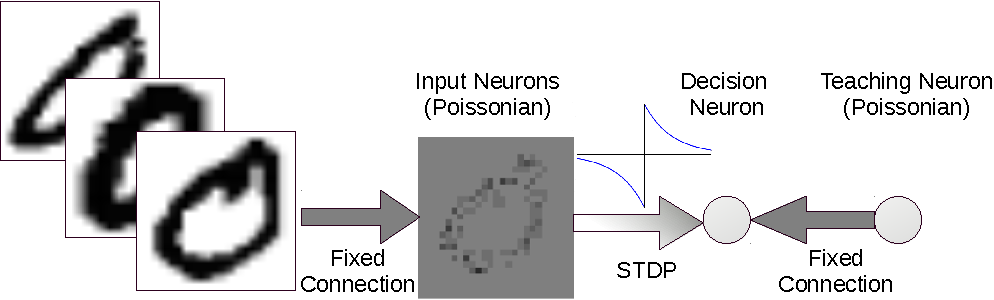
\includegraphics[width=0.48\textwidth]{images/training.pdf}
		} \\
		
		\centering
		
		\subfloat[Testing model of the spiking neural network.]{
			\label{Fig:test}
			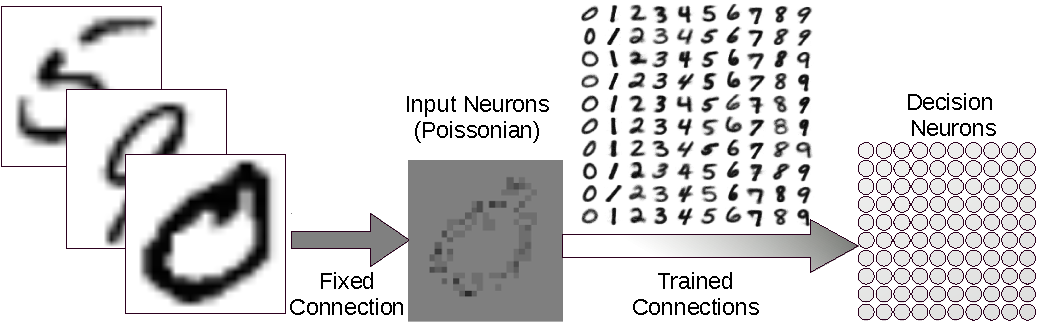
\includegraphics[width=0.48\textwidth]{images/testing.pdf}
		}
		
		\caption{The training and testing model of the two-layered spiking neural network.}
		\label{fig:model}
	\end{figure}
	\subsubsection{Testing}
	After training the weights of the plastic synapses are set to static, keeping the state of the weights at the last moment of training.
	%The weights were normalised after training and applied to the same network.
	The weak weights were set to inhibitory connections with an identical strength.
	%The output neurons inhibited all the other neurons as a winner take all circuit.
	The feed-forward testing network is shown in Fig.~\ref{Fig:test} where Poissonion spike trains are generated the same way as in the training with a total firing rate of $2,000$~Hz per image.
	The input neurons convey the same spike trains to every decision neuron through its responding trained synaptic weights. 
	Every testing image ($10,000$ images in total) is presented once and lasts 1~s with a silence of 200~ms between them.
	The output neuron with the highest firing rate decides what digit was recognized.
	Taken the trained weights from the NEST simulation, the accuracy of the recognition on NEST reaches 90.03\% with the standard configuration, while the result drops slightly to 89.97\% using SpiNNaker.
	In comparison, both trained and tested on SpiNNaker the recognition accuracy is 87.41\%, and with the same weights applied to NEST the result turns out to be 87.25\%.  
\section{Future Work: Spiking Deep Belief Net}
	In order to implement training of Spiking Deep~Belief~Networks~(SDBNs) on SpiNNaker, this paper studies the layer-by-layer training of spiking Restricted~Boltzmann~Machine~(RBM) of a DBN.
	The study starts from understanding the original problem, Products of Experts~(PoE), which was solved by using Contrastive~Divergence~(CD).
	It involves utilising Markov~Chain~Monte~Carlo~(MCMC) sampling to present the distribution of a certain untraceable high-dimensional probability model function, e.g. PoE.
	Among these sampling algorithms, Gibbs method is introduced and used in PoE problem.
	Instead of minimising the original objective function of Kullback-Leibler divergence, the contrastive divergence is exploited to solve PoE.
	Then the study continues on applying CD to RBM.
	Finally, on-line learning methods only spiking neurons used are explored to train spiking RBM.
	
	Need to draw a figure!
	And Gantt Chart.
	
\begin{appendices}
	\section{Thesis Outline}
	\label{app:thesis}
	The following section-level outline gives the planned thesis structure for this project.
	Sections which are reliant on upcoming work are indicated with a star (*);
	\begin{enumerate}
		\item Introduction
		\item Background
			\begin{enumerate}
				\item Neural Network on Image Recognition
				\item Neuron Models and Spiking Neural Network
				\item Spiking Neural Network Simulation
				\item Neuromorphic Simulators
			\end{enumerate}	
		\item Related Works
			\begin{enumerate}
				\item Vision Databases and Benchmarks
				\item Deep Neural Networks
				\item Spike-Based Image Recognition
				\item Real-Time Neuromorphic Vision System
			\end{enumerate}
		\item Benchmarking Spike-Based Visual Recognition
			\begin{enumerate}
				\item Database
				\item Evaluation Methodology
			\end{enumerate}
		\item Spiking Deep Belief Network
			\begin{enumerate}
				\item Restricted Boltzmann Machine  
				\item Deep Belief Network
				\item Spiking RBM and DBN *
%					\begin{enumerate}
%					\item Mean Field Theory
%					\item Synaptic Learning
%					\end{enumerate}	
			\end{enumerate}	
		\item Benchmarks
			\begin{enumerate}
				\item ConvNet without Learning
				\item STDP Learned 2-Layer Network
				\item Spiking DBN *
			\end{enumerate}	
		\item Discussions *
			\begin{enumerate}
				\item Benefits of Spikes
				\item Scalability of H/W SDBN
				\item Formalisation of SDBN
			\end{enumerate}					
		\item Future Work *
			\begin{enumerate}
				\item SDBN Toolbox on SpiNNaker
				\item Learning on Spiking ConvNet
				\item Video-Based Recognition and Benchmarks
%				\item Benchmarking Real-Time Neuromorphic Systems
			\end{enumerate}					
	\end{enumerate}	
\end{appendices}


\bibliography{ref}    % this causes the references to be listed
\bibliographystyle{ieeetr}
\end{document}